\chapter{Monitoring Application Energy Usage During Operation}
\label{chapter:monitoring}

\section{Introduction}

The energy usage of information and communications technology (ICT) systems is starting to receive much more attention that it has historically.  This is due to the sharply increasing demand for electricity to run the digital economy, with US datacenters alone consuming an estimated 91 billion kWh in 2013 and are expected to consume 140 billion kWh by 2020 \cite{delforge2014-datacentreenergy}.

Researchers have been working for some years to understand the energy demand of ICT systems and significant progress has been made in a number of areas.  At the macro level, we now have a fairly good understanding of how data centres use power and some understanding of how to reduce the amount of power required in the data centre environment \cite{dc4cities2014_dcmetrics}.  At the micro-level, there have been some promising steps in understanding how individual programs consume power, to the point where it is possible to quite accurately predict and compare the power consumption of different options for program implementation \cite{islam2016-energysoftwarefeatures}.

The problem for the software architect is that their interest sits between these two extremes as they need to understand the energy consumption at the overall application level rather than at the individual software module level or at the data centre level where many applications are consolidated.

The modern trend towards microservice-based systems \cite{wikipedia_microservices} makes things more complicated for the practitioner.  In theory it might be possible to use or adapt low-level energy estimation approaches to be useful with monolithic applications, this quickly becomes overwhelming with a microservice-based system, due to the number of possible pieces of the system that could be involved in processing a request or particular piece of workload.

In this chapter, we present the logical (i.e. technology independent) aspects of the design for a piece of technology that we have designed to address this problem by fairly allocating the energy usage of a host machine to the application elements running on it.  Using modern microservice and operating system technology including containers, tracing and resource monitoring, combined with energy statistics for a machine, we can provide the software architect, and also the host operator, with reliable estimates of the fair energy allocation of a machine's total consumption required to process requests for an application running on it.  This allows cost estimation but, more importantly from the software architect's perspective, the evaluation and exploration of architectural alternatives to minimise energy consumption.

The logical design in this chapter then forms the specification for our implementation of the ideas which we describe in Chapter \ref{chapter:implementation}.

\section{Motivation}

There are several reasons to seek a method of estimating energy usage by software applications, but two immediate motivating examples in our case are cost estimation and architectural evaluation.

Today, the energy consumption of an application is not taken into account when considering its cost to operate and so there is little motivation for the software architect to understand and minimize their application's energy footprint.  This prevents large possible reductions in energy usage and its associated resources of environmental impact and cost.

Even where the architect is interested in the energy usage of their application, no mainstream and practical approach for estimating the energy usage of software at the application level is available.  This means that for applications where a significant number of system elements are used to process a request, such as in a microservice-based system, it is theoretically possible to use program-level approaches to estimate the energy usage, but is complex enough that we do not believe that it would ever be done in practice.  This means that architects cannot evaluate the energy usage qualities of different architectural options that they are considering.

The specific advance achieved by this piece of work is the novel combination of application request level resource usage statistics, total host resource utilisation statistics, and host energy consumption to create an approach to fairly allocate the energy consumption of the host to the workload that ran on it at particular points in time.  This allows a fair, reliable and useful estimate of the energy usage that should be allocated to of specific requests made to the application.

The goal of this is to provide a practical approach for software architects to estimate the energy impact of their applications and to evaluate different architectural options in terms of their likely energy usage.

\section{Microservice-Based Systems}

The microservice architectural style \cite{richardson2018_microservices} is rapidly becoming a mainstream approach for building industrial software systems and it is systems build using this style that we are specifically interested in for this work.

A microservice-based system is made up of many small, encapsulated, network-connected services, rather than the more traditional approach of having a small number of large servers that aggregated many services (a so-called "monolith" \cite{mazlami2017_microservices_monoliths}).

For our purposes, the important characteristics of a microservice-based system are:

\begin{itemize}
\item The business logic in the system is implemented as a group of small, focused services, each performing one task, typically implementing a "bounded context" in Domain Driven Design terms \cite{evans2006_ddd}.
\item The services are as independent as possible and have well defined service interfaces and only interact through these interfaces.  Resources such as databases are owned by a specific service and are not accessed by other services (hence a microservice-based system will have many independent data stores rather than a single consolidated database used by many services).
\item Handling an incoming request for a system is likely to involve a set of cooperating services, with one handling the initial request and then calling other services in order to fulfil the request and provide a response.  Microservice-based systems often separate request-handling and domain services but we do not assume that this is necessarily the case.
\end{itemize}

Well designed microservice-based systems typically share other important characteristics \cite{newman2015_microservices}, such as independent build, test and deploy for each service, and interfaces defined using machine readable formats such as OpenAPI \cite{openapi2018} and RAML \cite{raml2018} but these other characteristics are not significant in the context of this work, and so we do not assume that they are present.

\section{Estimating Energy Usage}

As we investigated the problem of how to provide software architects, and other interested parties like data centre operators, with estimates of application level energy usage we identified a number of possible approaches.  

\begin{itemize}
\item Other researchers have tried to create entirely \emph{model based approaches} (such as \cite{seo2008-energystyle}) which can allow relative energy usage between different architectural structures to be estimated, but sidestep the problem of calculating actual energy values and require significant amounts of effort to create the models for non-trivial applications.

\item Other research projects have attempted to estimate architectural characteristics through \emph{event based simulation} \cite{grahn1998-energystyles} but creating event based simulation models is an unfamiliar process to many practitioners and again is significant amounts of effort for non-trivial systems.  It is also the case that existing research in this area has not yet investigated how to estimate energy consumption, but rather has focused on other architectural qualities such as performance.

\item At the \emph{micro-measurement level}, sophisticated approaches have been designed to estimate energy consumption for individual algorithms or programs \cite{noureddine2016-jolinar} with a high degree of success.  However these approaches rely on a highly controlled execution environment for the code being measured and access to low-level hardware state metrics, such as processor frequency statistics, in order to deal with the complex power characteristics of modern computing hardware.  While these models and tools are undoubtedly useful in the right situation, they are not practical tools for measuring the energy usage of a large-scale modern distributed application.

\item We explored whether we could combine the \emph{micro-measurement} approaches with \emph{application-level resource usage estimation} and produce meaningful energy estimates for the application-level workload.  However we found that approaches like Jolinar are not effective unless the low-level hardware state metrics can be provided and this wasn't practical in large distributed execution environments such as those used by microservice-based systems.

\end{itemize}

Having considered these options and realised that each of them had severe practical limitations, we shifted our focus slightly and reconsidered the goal of the work.  The problem we aimed to solve was to provide software architects and other interested parties with information on how to improve the energy efficiency of their applications.  The solution we identified to this problem was to shift our  goal from precisely estimating the \emph{actual} energy usage of a distributed application to estimating the \emph{fair allocation} of energy consumption to the application.  This is a useful goal because it allows service providers (such as cloud or hosting operators or data centre operators) to understand how to fairly allocate the cost of energy consumed by their infrastructure and it allows software architects to understand the energy consumption implications of their design decisions as a proporation of real energy cost, rather than simply a theoretical ratio between two design options.

Our approach assumes that the energy consumption of the execution platform that the application is executing on is available to the energy calculation process and uses this, along with the total resource usage consumption of the execution platform and the resource usage of the application components, to allocate the platform energy consumption to the different application elements running on it.  By tracing the execution of inbound requests across application elements, this allows us to allocate energy usage to specific requests and so compare the energy efficiency of different parts of a system, different workloads and different system design options.

Estimating energy usage at the application level is a complex process and so it is important to be clear how the calculation will be performed before trying to design an implementation of it.

There are five quite distinct parts to the problem:

\begin{itemize}

\item \emph{Identification of service elements involved in processing a request}.  Processing a request in a modern distributed system will often involve a chain of service calls between the services that comprise the system logic.  We assume that the implementation of the services is under the control of those wishing to estimate energy consumption.

\item \emph{Identification of the processing periods attributable to a request}.  Once we know the system elements involved in processing a particular request, we need to identify when the element was performing work on behalf of the request.

\item \emph{Resource usage of the request}.  Given the system elements involved in processing a request and the periods when they were active, on behalf of the request, we need to estimate the runtime resources consumed by the system elements during these periods.  The resource consumption we need to estimate is primarily the amount of CPU consumed (for reasons we will explain later) although the amount of active memory in use, the number of network i/o bytes sent and received, and the number of disk i/o bytes read and written are also typically available from modern operating system and container platforms.

\item \emph{Estimation of resource and energy usage of the underlying host machine}.  Our aim is to fairly allocate the energy used by a machine during a time window across the requests that were active during that period.  Hence we need to estimate the overall resource usage of the machine and the energy that it consumed as a result.  We also need a estimate of the PUE of the execution environment \cite{iso30134-pue}, to allow us to "load" the host's energy consumption to reflect the additional cost of the infrastructure (such as power transmission and cooling) that supports its operation.

\item \emph{Energy estimate of the request}.  Once we have the resource consumption metrics for a particular request, we then need to translate these into an estimate of the energy consumption that they imply.  We do this by establishing the percentage of overall machine resource utilisation that can be attributed to the request and then allocating the same percentage of energy usage of the underlying host to the request and then adjusting this by the PUE value for the execution environment (data centre) at the time of day that the request occured.

\end{itemize}

Each of these aspects of the problem is reasonably complex to solve, but luckily they can largely be solved independently, and once resolved, combined to achieve a reliable and fair energy allocation for each inbound request for a microservice-based system.  In the following sections of this chapter we discuss the "logical" design for a solution to each of these aspects of a problem.  This provides us with a largely technology independent design of the solution, which we then use as a specification for the technology specific design that we implemented, as described in chapter \ref{chapter:implementation}.

\section{Logical Design of an Energy Estimation System}

The functional design of a system to estimate energy usage for application requests (which we have dubbed "Apollo" - the Greek God of Prophesy, amongst other things) is shown in the informal block diagram in \ref{figure:logicaldesign}.

\begin{figure}
\centering
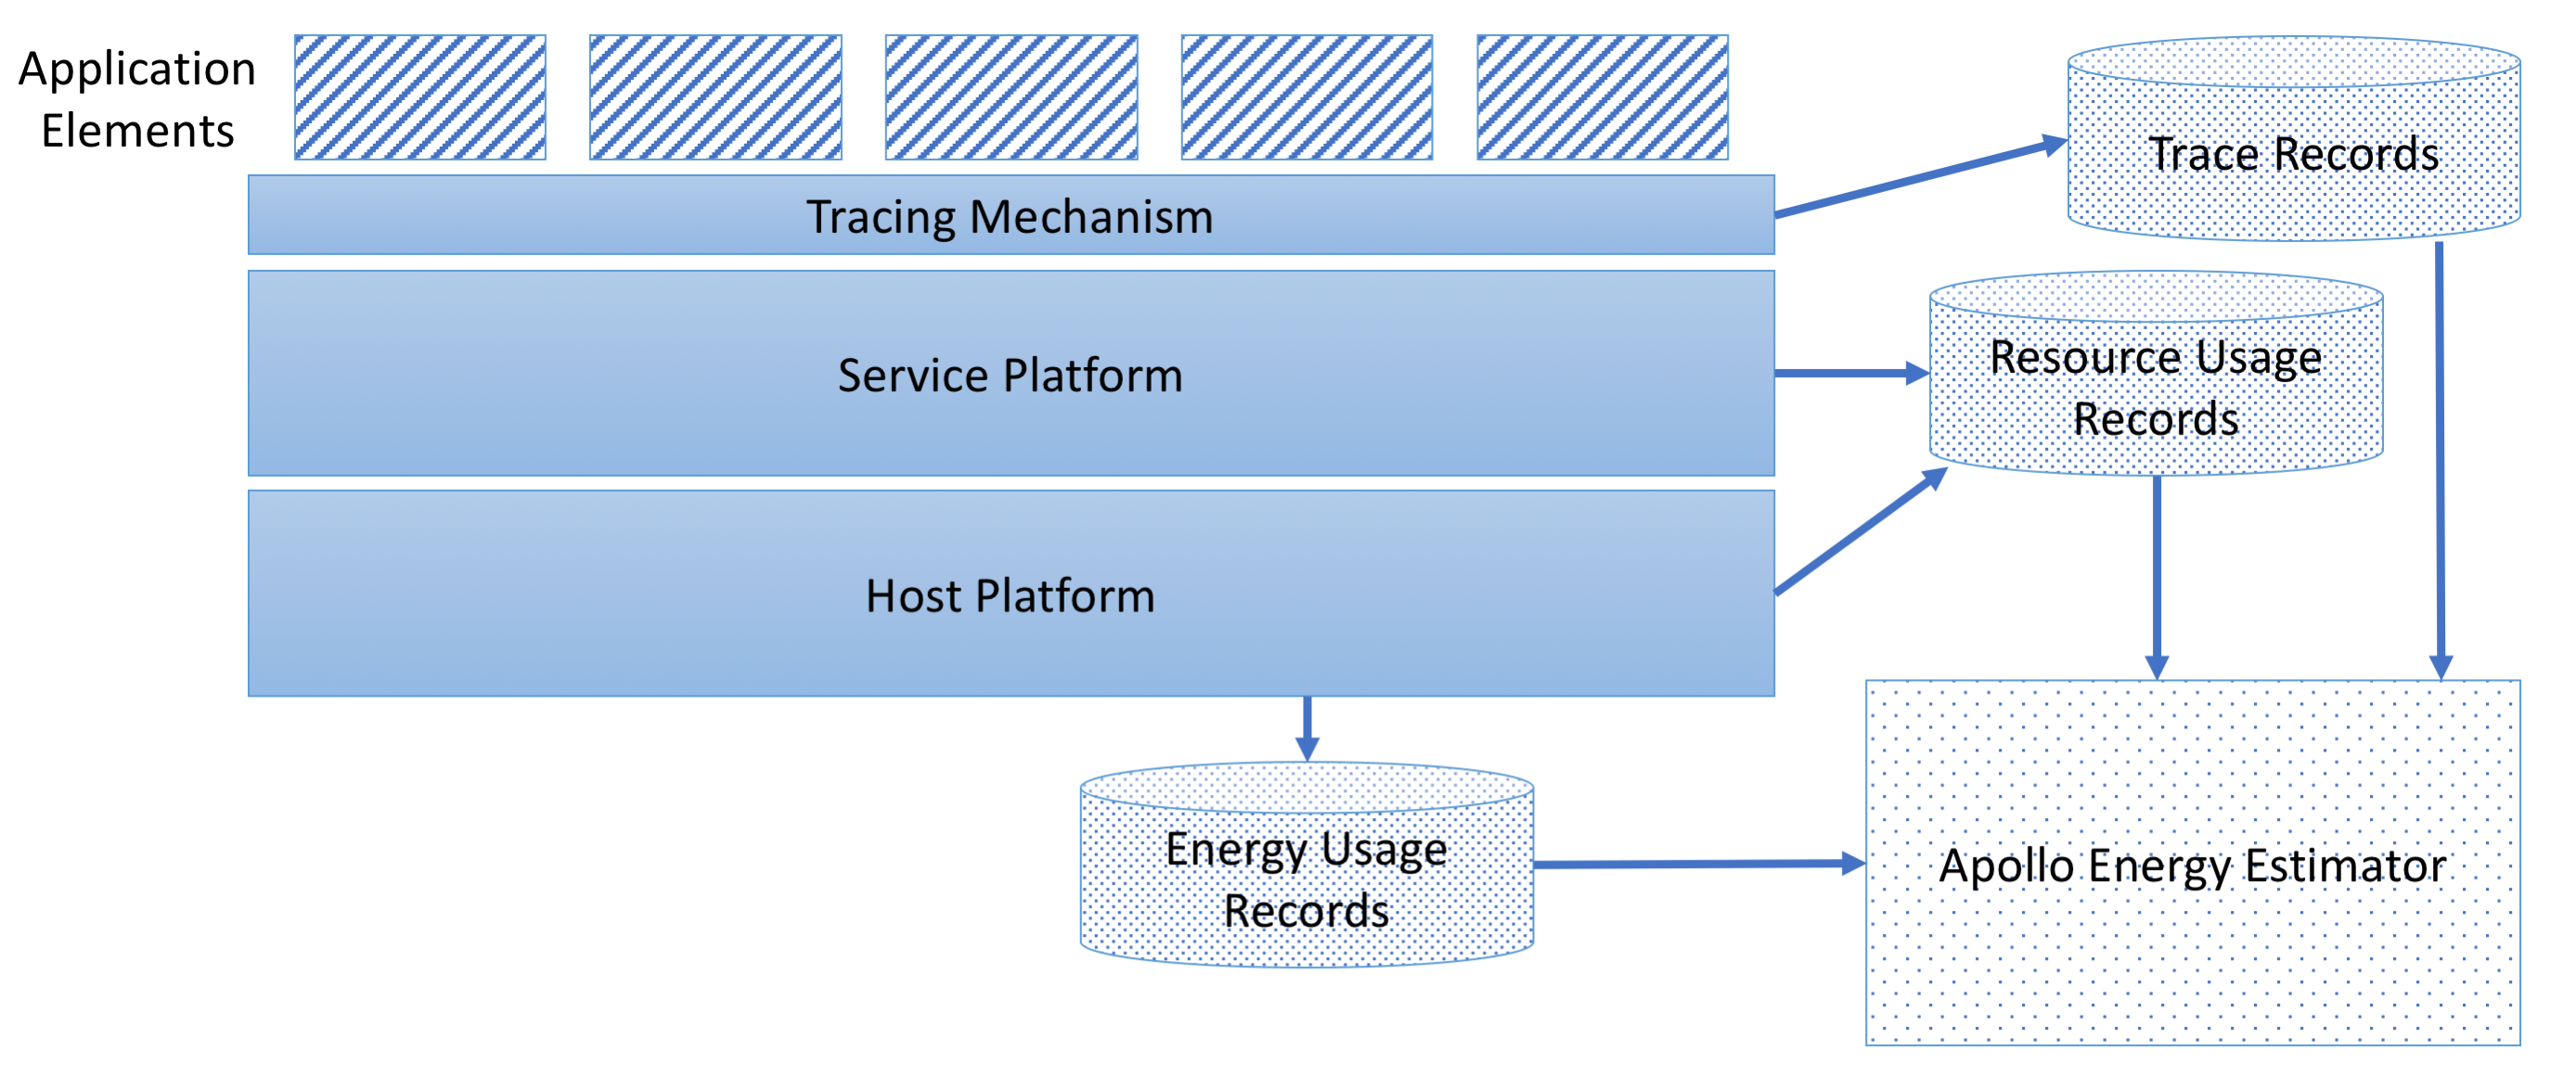
\includegraphics[width=\textwidth]{Figures/estimating-energy-logical}
\caption{Logical Design of the Energy Estimation System 'Apollo'}
\label{figure:logicaldesign}
\end{figure}

The elements in the diagram with solid fill are the underlying runtime platform and services, the diagonally hatched elements are the application under study, the densely-dotted elements are data, while the sparsely dotted elements are the Apollo energy estimation elements.

The elements of the system are briefly described below:

\begin{itemize}
\item \emph{Application Elements} are the architectural elements of the application which is being studied for energy consumption.  These are the main functional processing elements of the system, running in their own address space, providing a network interface to their services, invoked as part of request processing, with the implementation being under the control of the system owner who wants to estimate energy usage.  An example would be a request handling microservice to create an order.
\item \emph{Service Platform} is the system software which hosts the application components and can provide detailed measurements of their resource usage.  An example might be a PaaS platform like Cloud Foundry \cite{cloudfoundry2018}, a virtual machine, a modern operating system like Linux or a container platform like Docker \cite{docker2018} or Rkt \cite{rkt2018}.
\item \emph{Host Platform} is the hardware and operating system platform that provides the general computing platform that hosts the service platform and provides runtime statistics on the host's execution and energy consumption.  This is typically an Intel based server machine running a Linux or Windows operating system, or a virtualised version of them.
\item \emph{Tracing Mechanism}, which is key to our approach.  We require the ability to reliably and efficiently trace the architectural elements that were involved in handling a particular request for the system.  This tracing mechanism provides that ability, reporting the sequence of invocations of architectural elements and the time and duration of each.  Technology to allow this originated at Google \cite{sigelman2010-dapper} and has been implemented in open source projects such as Zipkin \cite{zipkin2018} and Jaeger \cite{jaeger2018}.
\item \emph{Resource Usage Records} is a database of resource usage statistics for all of the functional elements of the system, fed from the Service Platform and the Host Platform.  An example could be a regular database or a more specialised time-series database like Prometheus \cite{prometheus2018} or InfluxDB \cite{influxdb2018}.  The database is typically populated using a specialised statistics collection server like Telegraf \cite{telegraf2018} or cAdvisor \cite{cadvisor2018}.
\item \emph{Trace Records} is a database containing the request invocation traces from the Tracing Mechanism, which is likely to be a simple relational or document-oriented database, which the Tracing Mechanism writes its trace records to.
\item \emph{Apollo Energy Estimator} provides the key element of the energy estimation process, a calculator that works through the Trace Records and for each one, calculates which elements were active over which time periods, and uses the resource usage records to estimate the resource consumption of each request across the elements that were involved in processing the request.  These values are then compared with the overall host platform resource usage and the ratio of the values used to allocate the energy consumption of the host platform during the time period that the requests were active.

\end{itemize}

There are three key data structures in the design, which are critical to achieving the energy calculation, namely Trace Records, Resource Usage Records and Energy Usage Records.

\begin{itemize}

\item \emph{Trace Records} are created by the tracing mechanism and are used to record the invocation of system elements in processing a request.  There are two types of trace records, commonly referred to as Traces and Spans \cite{opentracing2018-traces}.  Common features of the two are the identity of the runtime element writing the record, the start time of the record and the end time of the record.  A "trace" record is written by the first element to handle an inbound request and its start time is when the request is received and its end time is when the response was dispatched.  A "span" record is written to record the invocation of another system element (i.e. service) by the original element handling the request and it has a "parent" attribute which indicates the trace it is part of.  Should an element \emph{e1} handle an inbound request and as part of processing it cause another element \emph{e2} to be invoked, then a trace record is written to record the execution of \emph{e1} and a span record is written, recording the execution of \emph{e2}, with the trace record as its parent.  Hence traces and spans are organized into a tree that mirrors the invocation structure of the request handling.  An example trace is shown in \ref{figure:span}.

\begin{figure}
\centering
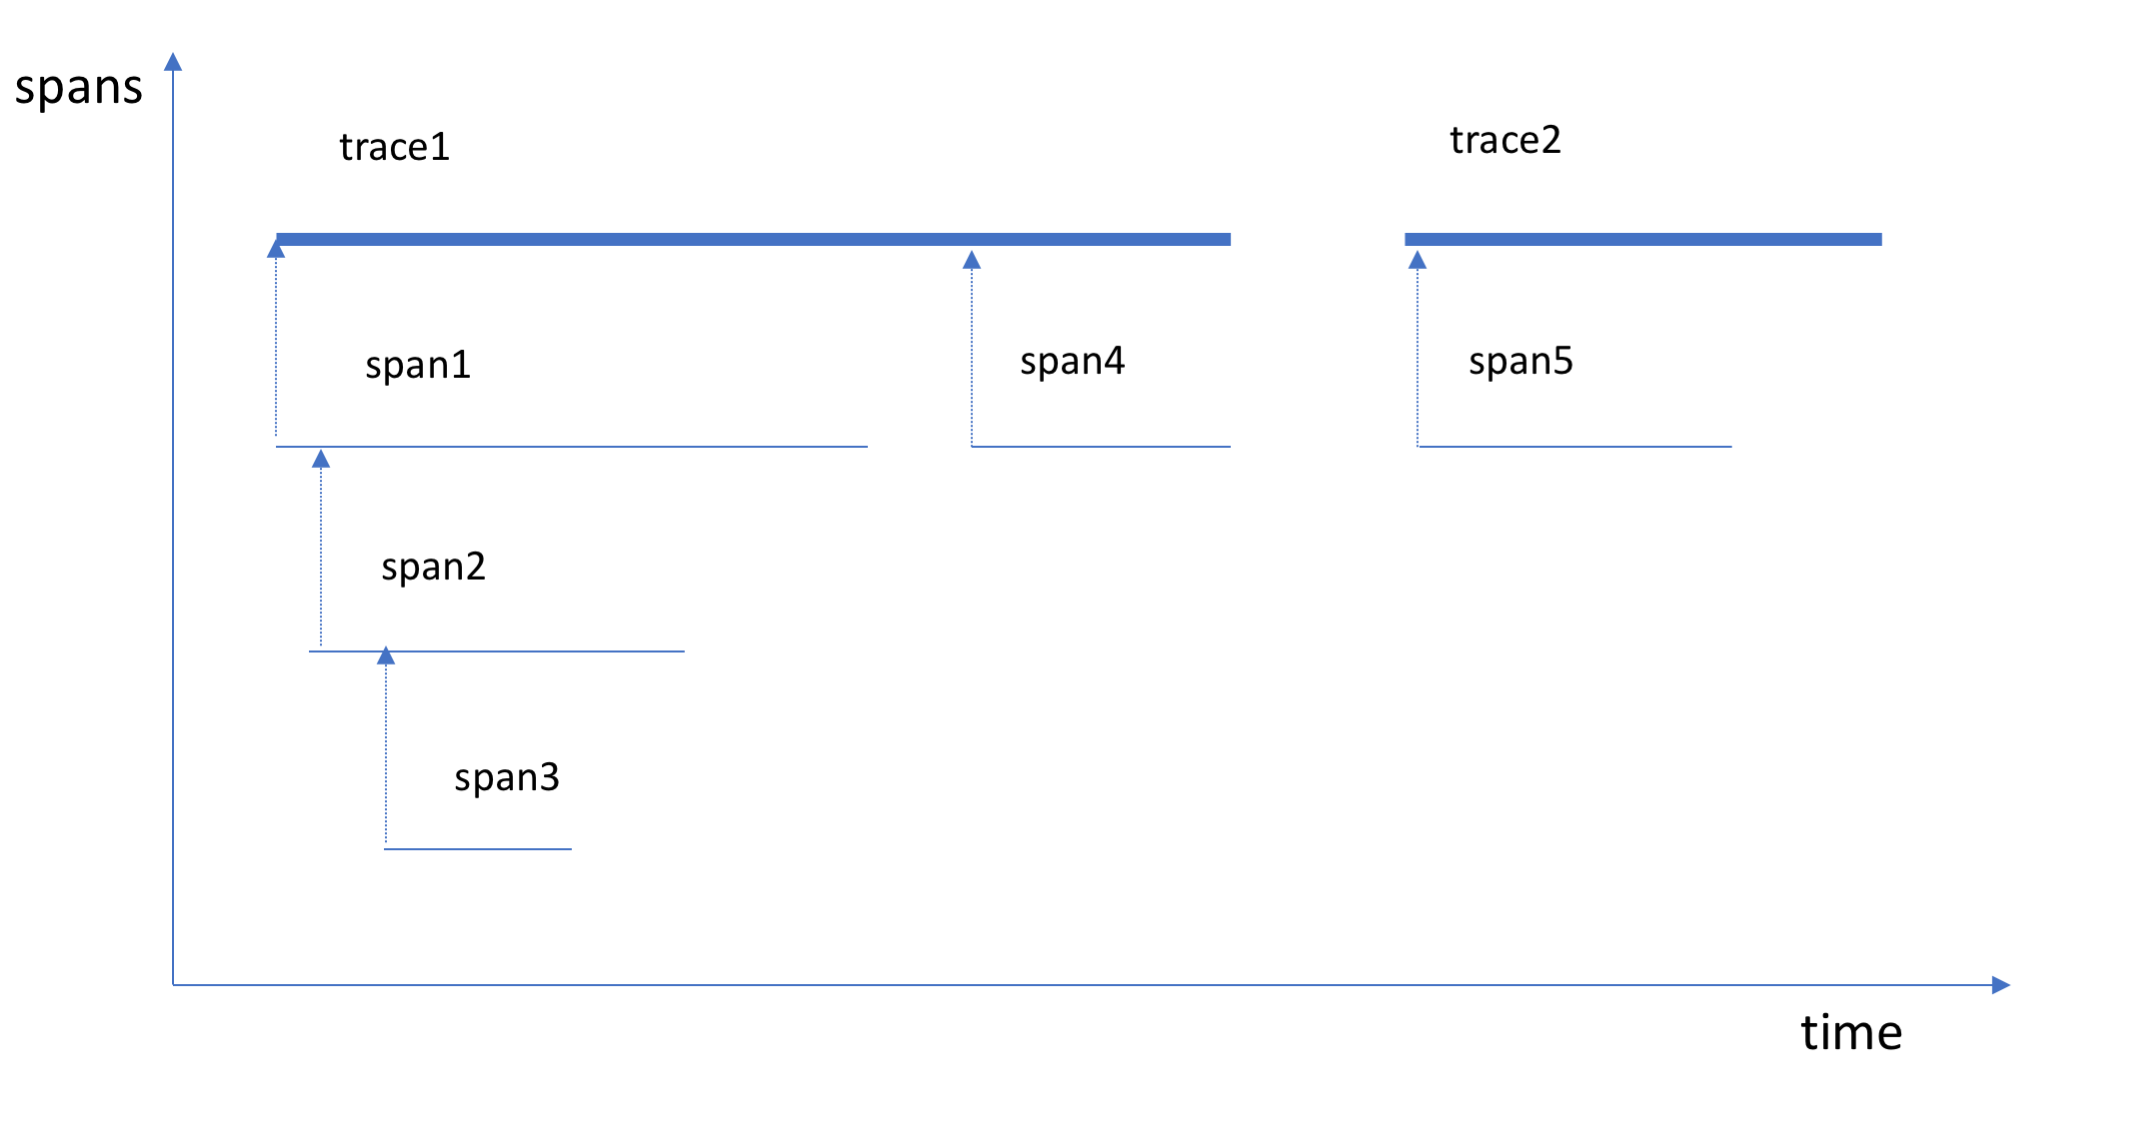
\includegraphics[width=0.75\textwidth]{Figures/estimating-energy-trace}
\caption{Example Execution Trace}
\label{figure:span}
\end{figure}

The figure shows two traces, representing requests, one after the other.  The traces are distinguished by not having parent spans, both traces have child spans, as indicated by the dotted arrows.  The y axis indicates invocation from top to bottom, the x axis indicates the passage of time.  The first request has two child spans, indicating that it invokes two other services.  Child span "span1" in turn invokes a third service, which invokes a fourth.  The second request invokes a single service.

\item \emph{Resource Usage Records} are generated by the runtime platform and the host platform and stored in a timeseries style database to allow the metrics for a particular runtime element during a specified period to be retrieved (e.g. metrics for process \emph{p1} for the 3 second period from 20171105T084512.500 to 20171105T084515.500 or metrics for the host \emph{h1} for the 12.5 second period from 20171105T084512.500 to 20171105T084525.000).  The metrics will be generated by the underling platforms at regular but arbitrary intervals and so this data store will need to interpolate between the available measurement points to get the resource usage for the requested time periods.  The metrics that both the runtime platform and the host platform will be assumed to create are CPU usage (in a hardware based measure such as "ticks" or a time based measure such as milliseconds), memory usage (in KB), disk IO (in KB) and network IO (in KB).  Absolute or cumulative measurements are both usable for our purposes.  At this stage, we assume that we can obtain a reliable measure of the resource utilisation of each architectural element of interest, without being concerned with how this is provided.  Mechanisms which could provide this data include a container system like Docker, an operating system's process statistics, an internal application monitoring system or even a virtual machine manager with each architectural element in a separate virtual machine.

\item \emph{Energy Usage Records} provide a history of the estimated energy usage of the host platform (that is the virtual or physical hardware and its operating system).  There are two varieties of energy usage record source that could be available to us depending on the situation.  In some cases, there will be physical energy usage records available from data centre infrastructure sources such as DCIM data collection platforms, like Sunbird \cite{sunbird2018} or Nylte \cite{nlyte2018}, which extract data from enterprise class hardware devices through a protocol like IPMI \cite{ipmi2013} (and increasingly its more secure and capable replacement, Redfish \cite{dmtf2018-redfish}).  These records can be fed into a timeseries database (similar to the one used for resource usage records) and queried directly.  In other cases, a model based approach can be used to simulate real power readings.  A model based approach can be used to produce workable estimates of energy usage at different points in time by using accurate power ratings for different hardware devices such as those reported through the use of the SPEC Power benchmark \cite{lange2009-specpower}.  These benchmark results provide accurate power consumption rates for specific pieces of hardware at different degrees of utilisation.  If we know what host platform is in use and have accurate host platform resource usage records (for CPU usage specifically) then these can be combined with the benchmark results to create a usable model-based estimate of energy usage of the underlying host at a point in time.

\end{itemize}

\section{Utilising Resource Usage Records}

Modern computing platforms like Linux and Windows provide detailed and comprehensive resource utilisation statistics that describe CPU utilisation (typically in terms of milliseconds or nanoseconds of CPU time used), disk i/o (in terms of read and write requests, blocks and bytes performed), memory utilisation (as KB of memory used over time) and network i/o (in terms of receive and transmit requests and bytes) \cite{unix_sar_command, windows_performance_monitor}.

When estimating energy characteristics of a workload, it is possible to measure the power consumption of a server via DCIM monitoring equipment or alternatively estimate power consumption of a server using a model based on reliable benchmarking.  However it is difficult to attribute the overall energy consumption of a server to the specific components within in.  While it is possible to obtain representative power specifications \cite{hitachi_drive_data_sheet} for individual components of enterprise class computing hardware, interpreting such specifications to produce accurate power consumption estimates is extremely difficult as they require a detailed understanding of the physical operation of the hardware element concerned during the period of interest (such as the frequency of the CPU or the amount of time that disks spend spinning at full speed during a particular measurement period).

As a result, we concluded that combining CPU, disk, network and memory utilisation statistics in order to produce power consumption estimates for a complex computing device, such as an enterprise server, was not a practical approach for anything other than the smallest laboratory examples and so was not suitable for the large scale enterprise use that we aspired to apply our work to.

However, it turns out that there is a solution to this problem, which is to use CPU utilisation as a proxy for overall server power consumption.  Previous research \cite{bashroush2018_hardwarerefresh} has shown that CPU utilisation is directly proportional to the power consumption of the server as a whole.  We have also investigated this and found that in more limited testing, in our specific environment, this relationship holds and CPU utilisation is a good proxy value for the relative power consumption of a server computer.  We discuss further validation of this finding in Chapter \ref{chapter:validation}.

This finding allows us to use CPU utilisation of the server host as a whole, compared to the CPU utilisation of the architectural elements used to process application requests, as a reliable proxy for the ratio of the energy consumption of the server to the energy consumption required to process application requests.

In the next section of this chapter, we explain how we calculate estimations of energy allocation for application requests.

\section{Calculating an Energy Allocation Estimate}

\subsection{Our Approach for Estimating Energy Allocation}

The key novel element in the system is clearly the Energy Estimator, which implements the processing required to fulfil the purpose of the system.  This element is a numerical calculator which combines data from the trace records, resource usage records and energy usage records in order to produce a reliable estimate of the amount of the energy of the underlying host which should be allocated to a specific request which the application under consideration has processed.

We illustrate the approach to creating an energy allocation estimate using the graph in Figure \ref{figure:cpuusage}, which shows the cumulative CPU usage over time for two architectural elements \emph{E1} and \emph{E2} along with the corresponding cumulative CPU usage for the host they are executing on.

\begin{figure}
\centering
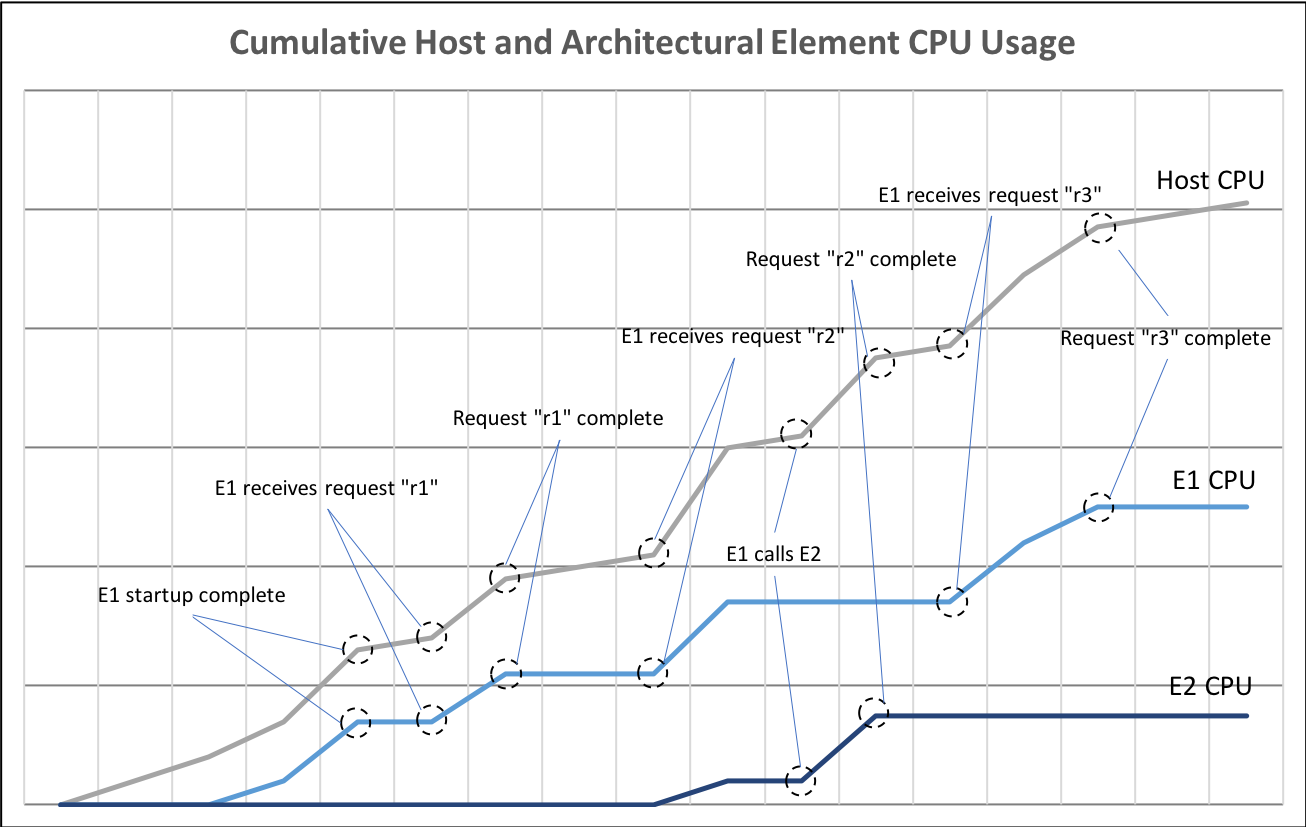
\includegraphics[width=1.0\textwidth]{Figures/estimating-energy-cpuusage}
\caption{Cumulative CPU for Request Handling}
\label{figure:cpuusage}
\end{figure}

The graph shows how CPU usage accumulates for an individual architectural element when it handles requests and how the CPU usage of the individual elements combine, along with other workload on the machine, to affect the host's CPU usage.

Starting from the left, the host and element \emph{E1} start up and use CPU during this process before becoming largely idle for a short period and so their CPU usage curves flatten.

Next element \emph{E1} receives a request, which we name \emph{r1}.  As can be seen, processing this request causes \emph{E1} to consume CPU rapidly, hence the CPU consumption curve becomes much steeper for a short period and the host's CPU usage curve follows a similar shape, reflecting the effect of \emph{E1}'s CPU usage on the host.  After request \emph{r1} has been processed, the CPU utilisation curves flatten again, reflecting the idle state that the application elements and the host are in.

The next part of the graph shows the arrival of another request, which we name \emph{r2}, processed by element \emph{E1}.  Similar to the previous request, this results in a short burst of CPU consumption by \emph{E1}.  However in this case \emph{E1} calls a second architectural element, \emph{E2} as part of the processing of the request.  At this point, this CPU consumption curve for \emph{E1} flattens as it is no longer consuming CPU, but \emph{E2}'s CPU consumption starts increasing rapidly for a short period.  Once \emph{E2} has completed processing, the host CPU curve flattens, indicating that request \emph{r2} has been processed.

Finally, element \emph{E1} receives a third request, which we name \emph{r3} and its CPU usage graph again becomes steep for a period as the request is processed.  Note that the CPU usage for processing request \emph{r3} is significantly greater than that which was recorded for processing \emph{r1} (and in fact \emph{r2}).  The host's CPU usage can be seen to increase in step, reflecting the impact of processing the request on the CPU usage of the host.

By comparing the shape of the host CPU usage graph to the usage graphs of the application elements it is possible to assess the amount of the host's CPU consumption which is attributable to the application elements.  In this example, the host CPU usage graph has quite a similar shape to application elements beneath it.  However careful inspection reveals that its slope is nearly always steeper than that of the application elements, reflecting the other workload that the host is undertaking in addition to that of the architectural elements.  

In this case, the fairly close match of the host usage curve to the application elements suggests that relatively little other workload is active on the host.  In the most extreme case, the host utilisation curve would be flat at the top of the graph, indicating close to 100\% utilisation and a very signifiant amount of other work being executed on the host in parallel with the application workload which we are studying.

It is this host CPU to application element CPU ratio which is key to our approach to allocating energy usage.  As explained above, we view CPU usage as a good proxy for the energy consumption of a host.  Therefore if an application's elements are consuming (say) 65\% of the host's CPU usage for a period, then we know that it is consuming roughly 65\% of the energy of the host during that period.

We use this insight as the key to designing an algorithm to allow us to estimate energy allocation for individual applcation requests, as explained in the next section.


\subsection{A Specification for Energy Allocation Calculation}
\label{subsection:calculation-specification}


We can express the specification for this algorithm as a series of simple equations as shown below.

As explained earlier usage records are \emph{Traces} which contain \emph{Spans}.  A \emph{Trace} represents an inbound request to the system and can be considered to be a tuple of the form 
\begin{equation}
Trace :: (tid, st, et, S)
\end{equation}
where $tid$ is a unique identifier for the trace record, $st$ is the start time of the trace, $et$ is the end time of the trace and $S$ is the set of spans that the trace contains.  

A span is a single invocation of an internal system element and so every trace contains at least one span (i.e. $\forall t : Trace \cdot t.S \neq \emptyset$) but most traces will contain a number of spans, related to each other, as illustrated in Figure \ref{figure:span}.  A span can be considered to be a tuple of the form
\begin{equation}
Span :: (tid, sid, st, et, a, pid)
\end{equation}
where $tid$ is the identifier of the trace this span is contained within, $sid$ is the unique identifier of this span, $st$ is the start time of the span, $et$ is the end time of the span, $a$ is the address of the architectural element that the span is invoking and $pid$ is the unique identifier of the parent span of this span, if there is one (this is an optional element in the tuple).

For both traces and spans times are assumed to be recorded to millisecond precision and are conventionally represented as the number of milliseconds since an agreed point in time, by convention 00:00:00 on the 1st January 1970 \cite{josey2004-ieee1003}.

The address of the architectural element can be any unique identifier which can unambigously identify an architectural element and can be captured reliably by the tracing system in use.  In practice, this is usually a network address of the form $ipaddr:port$ where $ipaddr$ is an IP version 4 address (e.g. 156.76.45.32) and $port$ is an IP network port (e.g. 9745).  However our approach does not require addresses of this form and other addressing and identification schemes could be accomodated if required.  We discuss this important detail further in Chapter \ref{chapter:implementation}.

Given these structural definitions we can now define how the energy estimation process should work.

Given a trace $t$ containing a span with ID $sid$ then let
\begin{equation}
a = t.S_{sid}.a
\end{equation}
\begin{equation}
st = t.S_{sid}.st
\end{equation}
\begin{equation}
et = t.S_{sid}.et
\end{equation}

Let us now consider how we describe the CPU usage of a span.  The process is illustrated in Figure \ref{figure:graph}.  The figure shows an example CPU usage statistic for a particular operating system process, captured as a cumulative usage value over time.  Points in time $t_{1}$, $t_{2}$ and $t_{3}$ are sample points, when the CPU usage statistic is reported.  Points $st$ and $et$ are the start and end times of the period we are interested in.  We indicate the value of the CPU usage statistic at a point in time using subscript notation where $C_{t_{1}}$ is the value at point $t_{1}$ and $C_{st}$ is the value at point $st$.

\begin{figure}
\centering
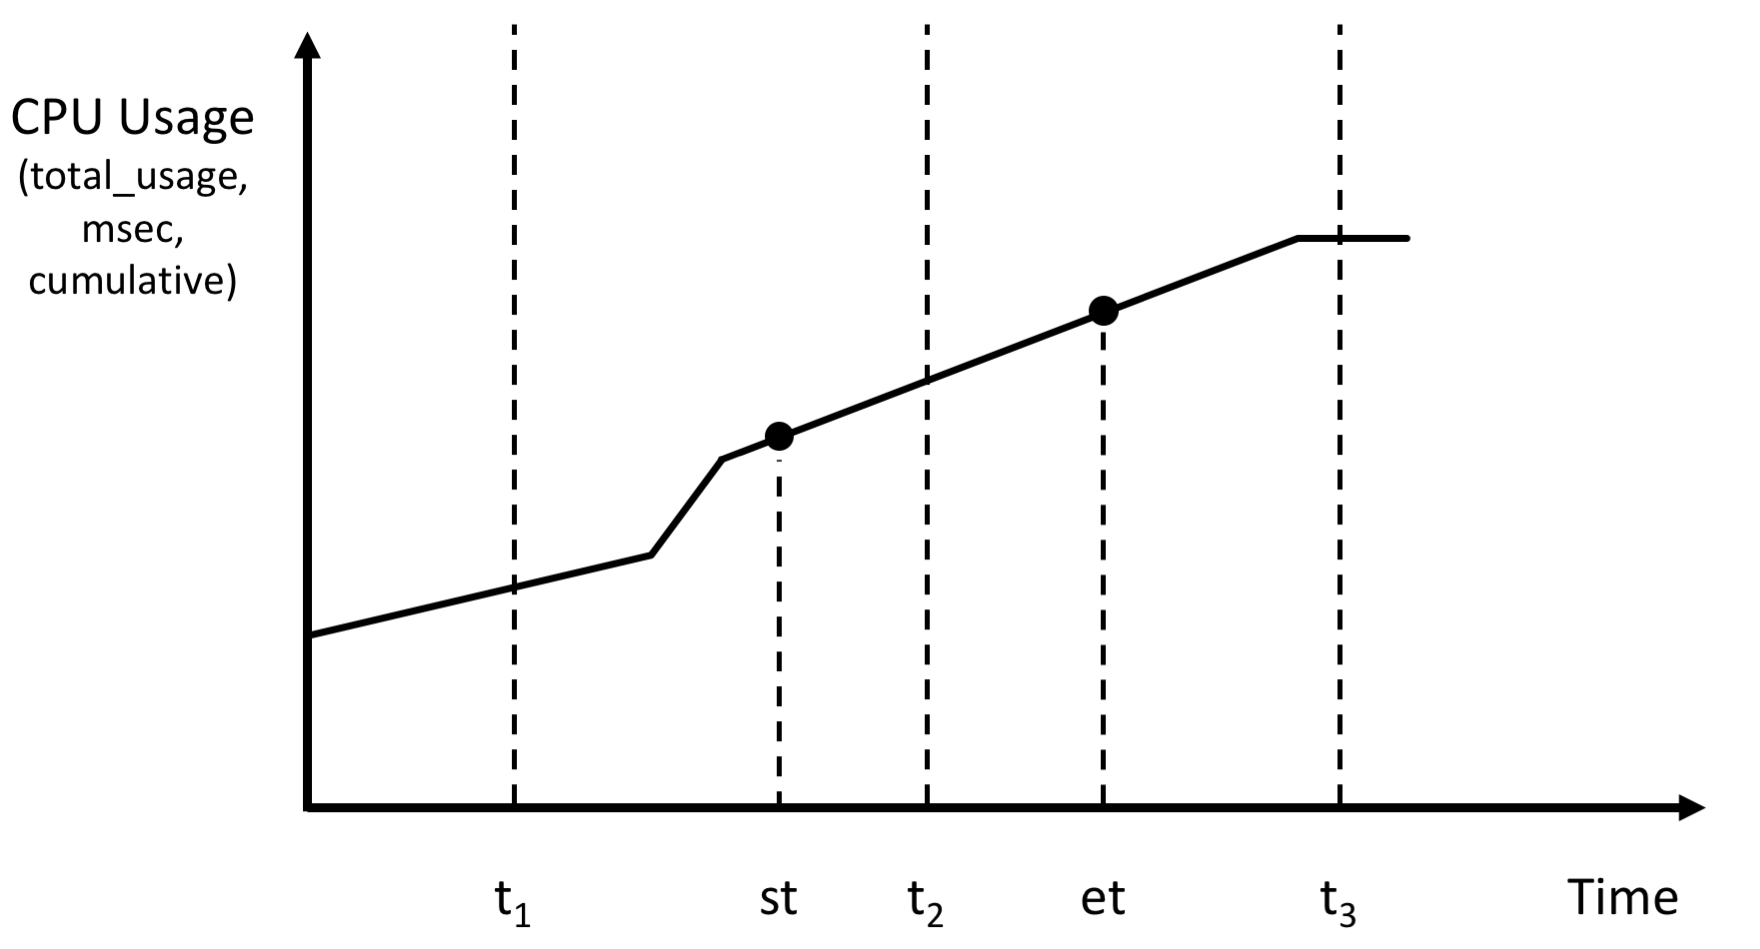
\includegraphics[width=0.75\textwidth]{Figures/estimating-energy-graph}
\caption{Cumulative CPU Usage Graph}
\label{figure:graph}
\end{figure}

Given $s$ is a span then we can describe the CPU usage of the span $s$ using the equations below, where $C_{s,t}$ indicates the cumulative CPU usage for the span at time $t$.

Let $C_{s, st}$ be the cumulative CPU usage for the span at point $st$ defined by
\begin{equation}
C_{s,st} = C_{s,t1} + \left( \frac{C_{s,t2} - C_{s,t1}}{t2 - t1} \times (st - t1) \right) 
\end{equation}

Let $C_{et}$ be the cumulative CPU usage at point $et$ defined by
\begin{equation}
C_{s,et} = C_{s,t2} + \left( \frac{C_{s,t3} - C_{s,t2}}{t3 - t2} \times (et - t2) \right) 
\end{equation}

Then the CPU usage of span $s$ can be defined as
\begin{equation}
C_{s} = C_{s,et} - C_{s,st}
\end{equation}

Given $h$ which is the host that a span executed on, and $st$ and $et$, which are the start and end times of a period respectively then we can describe the CPU usage of the host in a similar manner.

Let $C_{h, st}$ be the cumulative CPU usage for the host at point $st$ defined by
\begin{equation}
C_{h,st} = C_{h,t1} + \left( \frac{C_{h,t2} - C_{h,t1}}{t2 - t1} \times (st - t1) \right) 
\end{equation}

Let $C_{et}$ be the cumulative CPU usage at point $et$ defined by
\begin{equation}
C_{s,et} = C_{h,t2} + \left( \frac{C_{h,t3} - C_{h,t2}}{t3 - t2} \times (et - t2) \right) 
\end{equation}

Then the CPU usage of host $s$ between times $st$ and $et$ can be defined as
\begin{equation}
C_{h,st,et} = C_{h,et} - C_{h,st}
\end{equation}

Having estimated the CPU usage of the span during its execution period and the CPU usage of the host during the same period, we can use the ratio of the two, combined with the model-based or physical measurement estimates of the host's energy consumption over the same period.  Power indicates the rate of energy consumption at a moment in time and is a constantly and rapidly fluctuating value. We rely on averages of its value over time in order to find a representative value to use for our calculations.

In the situation where we have physical power metrics from the data centre infrastructure, then it is normal to find a Data Centre Infrastructure Management (DCIM) software platform deployed and we can extract power consumption metrics from this platform directly, using the API that such products expose. Different DCIM platforms offer different facilities and in some cases we might need to perform our own aggregation of device power readings in order to produce power consumption metrics suitable for our needs.  In other cases, the DCIM platform will have performed this aggregation and normalisation of the data already and we will be able to retrieve it via the API.  In ether case, the approach would be to produce a cumulative power usage metric for the hosts of interest in the managed environment, to allow a power usage average to be calculated in a similar way to the treatment of the cumulative CPU usage metric.

If a model based approach needs to be used then a slightly different it is calculated as follows:

Let $T_{h,st,et}$ be the total possible CPU consumption of host $h$ between start time $st$ and end time $et$.  Let $N_{h}$ be the number of CPUs that the host contains.

\begin{equation}
T_{h,st,et} = N_{h} * (et - st)
\end{equation}

Let $U_{h,st,et}$ be the percentage CPU consumption of host $h$ between start time $st$ and end time $et$.
\begin{equation}
U_{h,st,et} = \frac{C_{h,st,et}}{T_{h,st,et}}
\end{equation}

The power consumption estimate in watts, $P_{h}$, can now be extracted from the relevant SPECPower results for the model type of the host machine using $U_{h,st,et}$.

Let $E_{h,st}$ be the energy consumption (in joules) for the host between start time $st$ and end time $et$.
\begin{equation}
E_{h,st,et} = (et - st) \times 1000 \times P_{h}
\end{equation}


Given these supporting definitions we can now define the specification for the energy estimation process to be

\begin{equation}
E_{t} = \sum_{i=1}^{\#t.S} \left( \frac {C_{t.S[i]}} {C_{h,t.S[i].st,t.S[i].et}} \right) \times E_{h, st, et}
\end{equation}

The energy allocation for a trace is the sum of the energy allocations for the spans within it, which are each calculated as the ratio of the span resource usage to the host resource usage, during the span execution period, multiplied by the estimated host energy usage during the span execution period.

An algorithm which implements this specification will therefore allocate the energy used by the underlying host fairly across the application execution traces that it is executed for, so allowing fair comparisons to be made between different application requests to motivate design for energy efficiency and allowing recharging of energy costs in a fair and systematic manner.

\section{Implementing Apollo}

In this chapter we have explained the problem of providing energy estimates to a software architect and explored how this can be achieved in a realistic enterprise-computing environment through the use of a combination of resource consumption statistics, host energy consumption statistics and data centre efficiency factors.

So far our discussion has been largely implementation agnostic.  We have assumed the availability of the information we need, which presupposes a reasonably modern, mainstream enterprise application development and deployment environment (such as .NET on Windows or Java on Linux), but we have not limited or constrained our design by choosing specific technologies to use for data collection and analysis.  This means we have a specification for the software we need to build, which we could now implement using a choice of technologies for each part of the solution.

Realistically, when we choose technologies for each part of the solution they will solve parts of the problem for us and also constrain the solution and bring limitations and difficulties.  This is why presenting the implementation independent form of the design is important so that the underlying ideas can be explored and applied in a range of technology environments.  However we are aware that the design, and possibly its effectiveness, will be altered by the specific implementation choices we make when we build it.

In the next chapter we explain how we built a proof-of-concept version of Apollo, the technology choices we made, the problems we encountered and how we solved the problems to create a realistic and viable application energy calculator.

















